%%%%%%%%%%%%%%%%%%%%%%%%%%%%%%%%%%%%%%%%%%%%%%%%%%%%%%%%%%%%%%%%%%%%%%%%
% Escuela Politécnica Superior de la Universidad de Alicante
% Realizado por: Jose Manuel Requena Plens
% Contacto: info@jmrplens.com / Telegram:@jmrplens
%%%%%%%%%%%%%%%%%%%%%%%%%%%%%%%%%%%%%%%%%%%%%%%%%%%%%%%%%%%%%%%%%%%%%%%%

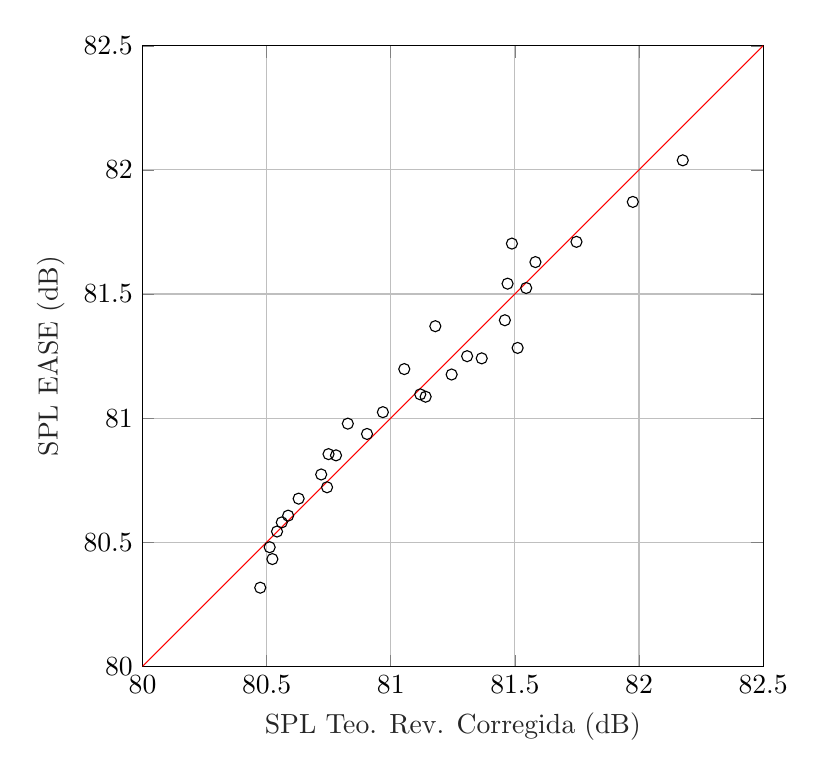
\begin{tikzpicture}

\begin{axis}[%
width=\textwidth,
height=0.65\textwidth,
at={(0\textwidth,0\textwidth)},
scale only axis,
xmin=80,
xmax=82.5,
xlabel style={font=\color{white!15!black}},
xlabel={SPL Teo. Rev. Corregida (dB)},
ymin=80,
ymax=82.5,
axis equal image=true,
%minor x tick num= 1,
%minor y tick num= 1,
%ytick distance=0.1,
ylabel style={font=\color{white!15!black}},
ylabel={SPL EASE (dB)},
axis background/.style={fill=white},
xmajorgrids,
xminorgrids,
ymajorgrids,
yminorgrids,
legend style={legend cell align=left, align=left, draw=white!15!black}
]
\addplot [color=black, only marks, mark=o]
  table[row sep=crcr]{%
80.5417583543006	80.5433304027162\\
82.1762817068517	82.0386358707718\\
80.5121065468405	80.4801041001578\\
80.5865014414949	80.6072443831041\\
80.7196944369790	80.7730979816846\\
80.9042299768582	80.9363543210067\\
81.1187342986678	81.0958466944594\\
81.3075137554158	81.2496512219242\\
81.4595895500597	81.3944484174868\\
81.5454353466553	81.5243050410068\\
81.5826814679269	81.6286916032713\\
80.6287695808118	80.6757816022743\\
81.4879654117737	81.7032602306948\\
80.4741526201567	80.3170447823861\\
80.5229843812398	80.4323281854646\\
80.5608617896108	80.5800232778857\\
80.7432806230875	80.7216052751135\\
80.7491795550527	80.8551228346567\\
80.8269321373207	80.9779007917098\\
81.1404282911666	81.0863383813745\\
81.2451624624217	81.1758102971935\\
81.3663646693337	81.2409187733041\\
80.7793706338611	80.8501127453048\\
81.5109656456417	81.2829074442554\\
80.9681387400627	81.0241339890186\\
81.0543473658963	81.1976817407895\\
81.1794515116566	81.3704539376178\\
81.4704552735545	81.5418269523107\\
81.7480751216254	81.7102885454161\\
81.9749784864042	81.8711413583681\\
};

\addplot [red,samples at={80,82.5}] {x};
\end{axis}
\end{tikzpicture}%